\section{Backtracking}

\subsection{17. Letter Combinations of a Phone Number}

\paragraph{\color{white} \colorbox{Mahogany}{Description}}
Given a digit string, return all possible letter combinations that the number could represent.

A mapping of digit to letters (just like on the telephone buttons) is given below.

\begin{figure}[ht]
    \centering
    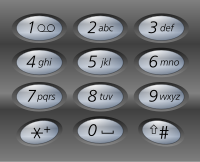
\includegraphics[width=5cm]{phone_number}
    \label{fig:phone_number}
\end{figure}

\paragraph{\color{white} \colorbox{OliveGreen}{Solution}}
$$f(s[1,\cdots,n])=\{m(s[1]],i)+f(s[2,\cdots,n])[j]|\text{ all possible } i,j\}$$
or
$$f(s[1,\cdots,n])=\{f(s[1,\cdots,n-1])[j]+m(s[n],i)|\text{ all possible } i,j\}$$
where $f(s)$ gives the set of possible letter combinations, $s$ denotes the digit string, $m(c,i)$ denotes the $i^{th}$ character of the key $c$.


\underline{Code Hints:}
\begin{itemize}
    \item We need to visit all leaf nodes, thus BFS (using a \mintinline{cpp}|deque<string>|), DFS/Backtracking (iteration or recursion) are all valid.
    \item Corner case for empty string input.
    \item If BFS, use \mintinline{cpp}|deque<string> result = {""};| to initialize the result (like a dummy head). Use \mintinline{cpp}|return vector<string>(result.begin(), result.end())|. to convert a queue to a vector.
\end{itemize}

\subsection{22. Generate Parentheses}

\paragraph{\color{white} \colorbox{Mahogany}{Description}}
Given n pairs of parentheses, write a function to generate all combinations of well-formed parentheses.

\paragraph{\color{white} \colorbox{OliveGreen}{Solution}}
\underline{Code Hints:}
\begin{itemize}
    \item We need to make sure left parentheses are fewer than $n$ and right parentheses are fewer than left parentheses.
    \item Corner case for \mintinline{cpp}|n==0| input.
\end{itemize}

\subsection{46. Permutations}

\paragraph{\color{white} \colorbox{Mahogany}{Description}}
Given a collection of distinct numbers, return all possible permutations.

\paragraph{\color{white} \colorbox{OliveGreen}{Solution}}
\underline{Code Hints:}
\begin{itemize}
    \item Because we need to traversal the whole tree until the leaf nodes are visited, returning intermediate results is not necessary. Thus, use \mint{cpp}|void recur(vector<ctx> &result, ctx &current, ...)| instead of \mint{cpp}|vector<ctx> recur(ctx &current, ...)|
\end{itemize}

\subsection{89. Gray Code}

\paragraph{\color{white} \colorbox{Mahogany}{Description}}
The gray code is a binary numeral system where two successive values differ in only one bit.

Given a non-negative integer n representing the total number of bits in the code, print the sequence of gray code. A gray code sequence must begin with 0.

\paragraph{\color{white} \colorbox{OliveGreen}{Solution}}
\underline{Code Hints:}
\begin{itemize}
    \item A bit of 1 with Exclusive Or can switch one bit, while a bit of 0 with XOR does nothing.
\end{itemize}

\subsection{79. Word Search}

\paragraph{\color{white} \colorbox{Mahogany}{Description}}
Given a 2D board and a word, find if the word exists in the grid.

The word can be constructed from letters of sequentially adjacent cell, where "adjacent" cells are those horizontally or vertically neighboring. The same letter cell may not be used more than once.

\paragraph{\color{white} \colorbox{OliveGreen}{Solution}}
\underline{Code Hints:}
\begin{itemize}
    \item Use \mint{cpp}|vector<vector<int>> path(board.size(), vector<int>(board[0].size(), 0));| instead of \mintinline{cpp}|set<pair<int, int>> path;| to store the path.
    \item Pruning at the beginning of the current recursion or before the next recursion.
\end{itemize}

\subsection{140. Word Break II}

\paragraph{\color{white} \colorbox{Mahogany}{Description}}
Given a non-empty string s and a dictionary wordDict containing a list of non-empty words, add spaces in s to construct a sentence where each word is a valid dictionary word. You may assume the dictionary does not contain duplicate words.

Return all such possible sentences.

\paragraph{\color{white} \colorbox{OliveGreen}{Solution}}
\underline{Code Hints:}
\begin{itemize}
    \item When the problem is huge and it may contain a lot of repeated pattern, Memoization + Recursion can be a good choice to avoid TLE.
\end{itemize}

\subsection{39. Combination Sum}

\paragraph{\color{white} \colorbox{Mahogany}{Description}}
Given a set of candidate numbers (C) (without duplicates) and a target number (T), find all unique combinations in C where the candidate numbers sums to T.

The same repeated number may be chosen from C unlimited number of times.

Note:
All numbers (including target) will be positive integers.
The solution set must not contain duplicate combinations.

\paragraph{\color{white} \colorbox{OliveGreen}{Solution}}
\underline{Code Hints:}
\begin{itemize}
    \item Divide the combinations into several groups according to the minimal index of the numbers they have. Thus, we do not need the sort before backtracking (divide the combinations according to the minimal number they have).
\end{itemize}